	\label{chap:dec}
	%Après avoir défini la relation interpersonnelle de dominance dans le chapitre \ref{chap:etat}, ainsi que sa manifestation dans l'interaction tant sur l'aspect verbal que non verbal, nous avons ensuite détaillé son impact sur les stratégies de négociations. 
	
	Ce chapitre introduit le modèle de décision d'un agent négociateur qui lui permet d'adapter sa stratégie de négociation à la relation de dominance qu'il vise à instaurer avec son interlocuteur. Dans la section 1, nous définissons les principes de décisions basés sur les comportements de pouvoir inspirés des travaux en psychologie sociale. Dans la section 2, nous présentons un premier modèle décisionnel utilisant des règles de décisions.  Pour ce modèle, nous nous sommes basés sur la structure d'arbres défini dans \emph{DISCO} \cite{rich09} et nous discuterons ses limites. Ensuite dans la section 3, nous présenterons notre modèle décisionnel final qui prends en compte les comportements de dominance de l'agent associés à ses préférences pour construire sa stratégie de négociation. Ensuite, nous présenterons deux études visant à valider le modèle décisionnel dans les deux cas d'interaction agent/agent et agent/humain.
	
	\section{Comportements de pouvoir et stratégies de négociation}
	\label{chap:domer}
	Comme nous l'avons présenté dans le chapitre \ref{chap:etat}, nous nous sommes essentiellement basés sur les travaux en psychologie sociale pour la définition de la dominance. 
	La dominance comme relation interpersonnelle est présentée comme la capacité à exprimer des comportements verbaux et non verbaux par lesquels  l'influence est atteinte. Prenant cette définition comme point de départ, nous nous sommes ensuite intéressé à la manifestation des comportements de dominance durant le processus de négociation et comment ces comportements influençaient les stratégies de négociations dans le contexte d'interaction humain/humain. 
	
	Dans ce qui suit, nous présentons \emph{trois principes} de comportements extraits des travaux en psychologie sociale qui ont étudiaient l'impact du pouvoir sur les négociateurs et leur stratégies.
	
	\begin{enumerate}
		\item \textbf{Niveau d'exigence et de concessions:} Les négociateurs dominants affichent un niveau d'exigence plus important comparés aux négociateurs soumis. Par ailleurs, les exigences des négociateurs soumis diminuent avec le temps. Ceci se traduit par des concessions plus importantes comparés aux négociateurs plus dominants. \cite{de1995impact}
		
		\item \textbf{Soi \emph{vs} autrui:} Les négociateurs soumis prennent en compte les préférences de leur interlocuteur dans la négociation, tandis que les négociateurs  dominants sont centrés sur eux-mêmes et s'intéressent uniquement à la satisfaction leurs propres préférences. \cite{fiske1993controlling,de1995impact}
		
		\item \textbf{Contrôle du flux de la négociation:}
		Les négociateurs dominant ont tendance à faire le premier pas et à prendre les devants dans la négociation \cite {magee2007domer}. Ils sont centrés sur l'avancement du processus de prise de décision, en prenant des décisions rapides \cite{zablotskaya2012relating}.
		A l'opposé, les négociateurs moins dominants visent à construire un modèle précis des préférences du partenaire de négociation. 
		Par conséquent,  ils posent plus de questions afin de collecter les informations nécessaires qui leurs permettent de prendre la décision la plus équitable(\emph{e.g}  faire des propositions)~\cite{de2004influence}. 
		
	\end{enumerate}
	
	
	Le but est de construire un modèle de décision capable d'illustrer ces comportements de dominance et par conséquent, adapter la stratégie de négociation en fonction de la dominance de l'agent.
	
	Dans ce qui suit nous présenterons le modèle décision de l'agent qui prend en compte la relation de pouvoir.
	
	
	\section{Règles de décision}
	Dans le cadre de cette thèse, nous avons construit un premier modèle de décisions composé de règles de décision modélisées sous forme d'arbres de dialogues. L'implémentation de notre système de dialogue est géré par le logiciel \emph{Disco}. Disco est une implémentation d'un ``collaborative discourse manager'' inspiré d'une théorie de dialogue collaboratif comme \emph{Collagen} \cite{rich1997collagen}. Disco est un système qui permet la génération de dialogues orienté tâches pour lequel il utilise le formalisme des \textbf{HTNs} (Hierarchical Task Networks) \cite{erol1994htn} pour la gestion des tâches. Il est implémenté avec le standard ANSI/CEA-2018 : chaque tâche est définit avec des préconditions, des effets et des postconditions. Les tâches sont regroupées par \emph{recettes} munies de conditions d'applicabilité.
	
	De plus, \emph{Disco} a été étendu avec un module génération d'arbres de dialogues afin de communiquer et collaborer avec l'utilisateur pour la réalisation des tâches. Ce module est nommé Disco for Games (D4g) et permet de définir des sémantiques d'actes de dialogue. D4g est déjà fourni avec un ensemble d'actes de dialogue.
	
	Nous avons complété ce système avec les actes de dialogues présenté dans la section \ref{sec:communication} afin qu'il puisse supporter la négociation sur les préférences.
	
	Pour chaque acte de dialogue que l'agent reçois, nous modélisons l'ensemble des réponses que l'agent peut sélectionner. Par exemple, suite à un acte \emph{Propose} énoncé par l'utilisateur, l'agent peut répondre par un \emph{Accept}, un \emph{Reject} ou un autre \emph{Propose}. Par exemple:
	("User: Je propose que nous allions dans un restaurant Chinois. 
	
	Agent: je propose que nous allions plutôt dans un restaurant Japonais"). 
	
	Chaque branche est définie avec des conditions d'applicabilités pour décider quelle réponse est adoptée. 
	Ces conditions prennent en compte la dominance de l'agent en plus du contexte courent de la négociation. Dans l'exemple précédent, l'agent doit être dominant pour répondre à un Propose par un autre Propose. 
	
	
	\subsection{Sélection de l'acte de dialogue}
	Nous avons initialisé l'agent avec un comportement de pouvoir parmi trois types de comportements de pouvoir inspirés de la littérature en psychologies social.  L'agent peut suivre un comportement \emph{dominant, soumis} ou \emph{neutre}. 
	
	En fonction de l'acte de dialogue que l'agent reçoit, nous générons un ensemble de réponses possibles. Chaque réponse dépend du pouvoir de l'agent. Le système de dialogue offre à l'utilisateur la liberté de choisir n'importe quel acte de dialogue pour son tour de parole. Disco déroule alors l'arbre de dialogue correspondant de gauche à droite (en commençant par la branche la plus à gauche). La première branche applicable rencontrée est directement exécutée sans vérifier les branches restantes.
	
	Notons que dans la suite, chaque arbre de dialogue est défini avec une condition de sortie qui clos la négociation avec un échec. Cette dernière est activée seulement par agent \emph{dominant} dans la situation où toutes les valeurs restantes ne sont pas acceptables. 
	
	\subsubsection{AskPreference}
	A la réception d'un \emph{AskPreference}, l'agent répond en exprimant ses préférences sur la question demandée comme présenté dans la figure .. .
	
	\subsubsection{State Preference}
	Le comportement standard qu'un agent adopte à la réception d'un \emph{StatePreference(v)} est de donner son opinion sur la valeur exprimée (c-à-d que l'agent calcule la valeur de satisfiabilité de \textit{v}). Cependant, si l'agent a déjà exprimé ses préférences sur ces valeurs, il va vouloir choisir un autre acte de dialogue en fonction de la relation sociale:
	\begin{itemize}
		\item \emph{Propose(x)}: Si la valeur exprimée par l'utilisateur est acceptable (voir figure \ref{pseudo}) pour l'agent, il va proposer de choisir cette valeur. Ce comportement relate le principe 1.
		\item \emph{Propose}: Si le nombre de \emph{StatePreferences} autorisé est atteint (voir figure \ref{alg:maxtours}), l'agent doit respecter le principe 3 et faire évoluer la négociation. La valeur proposée doit respecter les préférences de l'agent. 
		\item \emph{StatePreference}: l'agent est \emph{neutre}, il va vouloir exprimer ses préférences afin de construire une meilleure connaissance.
		\item \emph{AskPreference}: l'agent est \emph{soumis}. Dans le cas où toutes les valeurs du critères courent ont été discutés, l'agent va respecter le principe 3 et faire évoluer la négociation en ouvrant la discussion sur un autre critère.
	\end{itemize}
	
	\begin{figure}[]
		\begin{algorithmic}[1]\small
			\Function{MaxStatements}{}
			\State $nbTours$ = Nombre de \emph{StatePreferences} exprimés successivement.
			\State $maxTours$ 
			\If{($dominant$)} 
			\State $maxTours = 1$
			\EndIf
			\If{($peer$)} \State $maxTours = 2$
			\EndIf
			\If{($soumis$)} 
			\State $maxTours = 4$
			\EndIf
			\State $retrun$ $nbTours\geq maxTours$
			\EndFunction
		\end{algorithmic}
		\vskip 8pt
		\label{alg:maxtours}
		\caption{Maximum de tours de \emph{StatePreference} autorisé en fonction du pouvoir de l'agent}
	\end{figure} 
	\subsubsection{Propose}
	A la réception d'un \emph{Propose} comme présenté dans la figure ..., l'agent choisit sa réponse en fonction de l'\emph{acceptabilité} de la proposition.
	Nous avons écrit l'algorithme d'acceptabilité afin qu'il s'adapte à la valeur de pouvoir de l'agent. Ce choix permet de refléter les comportements du principe 2 \emph{niveau d'exigences et concessions}.
	
	En effet, au fur et à mesure que la négociation évolue, l'agent va faire des concessions sur certains critères. Par exemple, il peut considérer que le critère de \emph{localisation} n'est plus important pour le choix d'un restaurant. Par conséquent, il considérera que toute valeur de \emph{localisation} est désormais \emph{acceptable}.
	
	Par ailleurs, la notion d'exigence apparaît dans l'algorithme ci-dessous. Si l'agent est \emph{dominant}, l'ensemble de valeurs acceptables est plus restreint qu'un agent \emph{soumis}.
	
	\begin{figure}[]
		\begin{algorithmic}[1]\small
			\Function{isAcceptable}{$proposal$}
			\If{(type de $proposal$ n'est pas un critère important)} 
			\State return $true$
			\EndIf
			
			\State List = trier les valeurs par ordre décroissant de préférences
			\If{($dominant$)} 
			\State $return$ index($proposal$)< $size(List)/2$
			\EndIf
			\If{($soumis$)} 
			\State return $return$ index($proposal$)< $size(List)/4$
			\EndIf
			\EndFunction
		\end{algorithmic}
		\vskip 8pt
		\label{pseudo}
		\caption{Calcul d'acceptabilité d'une proposition $value$}
	\end{figure} 
	
	
	L'arbre de décision produit pour répondre à un \emph{Propose(p)} est présenté dans la figure .... 
	\begin{itemize}
		
		\item  \emph{Accept(p)}: Si la proposition \emph{p} est acceptable, l'agent doit exprimer un \emph{Accept(p)}. Sinon, l'agent doit faire évoluer la négociation pour trouver un meilleurs compromis. En fonction de la relation de pouvoir l'agent choisit un acte de dialogue spécifique.
		\item \emph{Ask :} l'agent \emph{soumis} va suivre les comportements décrit dans les principes 1 et 3. En effet, il va essayer de collecter plus de connaissances sur les préférences de l'autre et ainsi prendre en compte ses préférences. De plus, en vue du principe 2 qui affirme qu'un agent soumis doit faire des concessions, l'agent soumis n'est pas autorisé à exprimer plus d'un nombre de rejets successifs.  
		\item \emph{Reject :} l'agent qui n'est pas dominant (\emph{i.e. soumis ou neutre}) rejete une proposition qui n'est pas acceptable.
		\item \emph{Propose :} suivant le principe 3, l'agent \emph{dominant} fait évoluer la négociation en proposant une autre valeur qui respecte mieux ses préférences. 
	\end{itemize}
	
	
	
	\subsubsection{Accept }
	A la réception	d'un \emph{Accept}, nous séparons deux cas de réponses en fonction du type de la valeur acceptée $v$.
	Premièrement, $ v \in \mathcal{O}$ une \textit{option}, l'agent clos la négociation par un \emph{succès}.
	Sinon, $v \in C_i$ est une valeur de critère, l'agent entame la négociation sur un autre critère et sa réponse sera choisie en fonction de la relation de pouvoir à exprimer.
	
	\begin{itemize}
		\item \emph{Propose}: La condition d'applicabilité pour cet acte de dialogue dépend du pouvoir de l'agent. Un agent \emph{dominant} entamera la négociation sur le nouveau critère en proposant une valeur qui respecte ses préférences. Cependant, un agent \emph{soumis} n'est autorisé à faire une proposition que s'il a des connaissances sur les préférences de l'autres,  communiqués par des \emph{StatePreferences}, qui lui permettront de prendre une décision équitable. cet algorithme traduit les comportements présentés dans les principes 1 et 3. 
		
		\item \emph{AskPreference}: Comme présenté dans le principe 3, l'agent est \emph{soumis} collecte le plus d'informations possibles sur les préférences de son interlocuteur. 
		\item \emph{StatePreference}: L'agent est \emph{neutre} ouvre la négociation en communiquant ses préférences sur le nouveau critère à discuter. 
		
	\end{itemize}
	
	%				\begin{figure}[]
	%					\begin{algorithmic}[1]\small
	%						\Function{CanPropose}{}
	%						\If{($dominant$)} 
	%						\State return $true$
	%						\EndIf
	%						
	%						\State 
	%						\If{($soumis$)} 
	%						\State l'agent a des connaissances suffisantes sur les préférences de l'interlocuteur
	%						\State return $true$
	%						\EndIf
	%						\EndFunction
	%					\end{algorithmic}
	%					\vskip 8pt
	%					\label{alg:canPropose}
	%					\caption{Calcul d'acceptabilité d'une proposition $value$}
	%				\end{figure}
	%				
	
	\subsubsection{Reject}
	Suite à un \emph{Reject}, l'agent choisis une réponse en suivant les trois principes comme présenté ci-dessous:
	\begin{itemize}
		\item \emph{AskPreference}: Si la proposition d'un agent \emph{soumis} est rejetée, il va considérer qu'il n'avait pas assez de connaissances pour prendre une bonne décision. Pour compenser, il va demander à l'utilisateur ses préférences sur des valeurs qu'il ne connaît pas déjà. 
		
		\item \emph{Propose}: Suivant les principes 1 et 3, l'agent \emph{dominant} fait avancer la négociation en proposant de nouvelles valeurs. Cependant, si la valeur rejetée se trouve être la valeur qu'il préfère le plus, il va refuser de concéder et donc proposer la valeur encore une fois. Ce comportement est fidèle au principe 2. 
		
		\item \emph{StatePreference}: l'agent \emph{peer} continue la négociation en exprimant ses préférences sur d'autres valeurs. 
	\end{itemize}	
	%----------------------------------------------------------------
	
	\subsubsection{Exemple}
	Nous présentons un dialogue généré en utilisant notre modèle de dialogue. Deux agents\textit{A} et \textit{B}
	
	
	A: "Let's go to a Chinese restaurant."
	
	B: "I like Italian more than Chinese restaurants."
	
	A: "Let's go to a quiet restaurant."
	
	B: "I don't like quiet restaurants."
	
	A: "Let's go to a cheap restaurant."
	
	B: "Do you like quiet or lively restaurants? "
	
	A: "I like quiet restaurants."
	
	B: "I like lively restaurants."
	
	A: "Let's go to the Samura restaurant. It's a lively, cheap Japanese restaurant."
	
	B: "What kind of cuisine do you like?"
	
	A: "I like Chinese restaurants."
	
	B: "I like Italian restaurants."
	
	A: "Let's go to the Dragon restaurant. It's a lively, cheap Chinese restaurant."
	
	B: "Okay. Let's go to the Dragon restaurant."
	
	A: "Okay. I'll call to book a table."
	
	
	\subsection{Evaluation du modèle}
	\subsection{Limites des arbres de dialogue}
	Parler de l'étude qui a montré une ambiguïté dans la perception des comportement et la capacité à isoler l'impact de chaque principe sur la prise de décision
	
	Comportement incongrue ou non attendue.
	
	Situation de \textit{breakdown}, du a une modélisation manuelle, nous avions rencontrer des situations où aucune condition d'applicabilité n'étaient vrai. 
	
	Pour toutes ces raisons, nous avons repenser notre solution pour qu'elle soit plus fidèle aux principe de négociation et qu'elle puisse refléter les comportements de pouvoir. 
	
	\section{Modèle de décision basé sur les comportements de pouvoirs}
	
	Nous proposons un modèle computationnel de décision, qui reprend les trois principes de pouvoir dans le modèle décisionnel de l'agent. 
	A cause de la rigidité des arbres de dialogues, nous adaptons la solution afin qu'elle soit plus flexible de l'utilisateur et surtout afin que les comportements de pouvoir soient plus saillant dans les décisions de l'agent.
	
	Par conséquent, nous présentons dans ce qui suit, l'adaptation algorithmique de chaque principe de dominance extraits de la psychologie sociale.
	
	L'agent est défini avec une valeur de dominance $dom \in [0,1]$ qui représente sa position de dominance dans l'interaction, tel que plus $dom$ se rapproche de 1, plus l'agent est dominant. 
	
	\subsection{Principe 1: Niveau d'exigence}
	
	Selon notre premier principe, le niveau d'exigence devrait être plus important chez les agents dominants. Cependant, au cours d'une négociation collaborative, les deux négociateurs sont amenés à réduire leur niveau d'exigences parce qu'ils veulent parvenir à un accord. Les psychologues observent des concessions plus importantes pour les négociateurs soumis. 
	
	Nous avons implémentés ces comportements en deux phases. En effet, afin de modéliser la différence d'exigence dans la négociation, nous avons implémenté une fonction de satisfiabilité qui prend en compte la valeur de pouvoir initiale de l'agent. 
	
	Soit $S$ l'ensemble de valeurs satisfiables pour l'agent. Ceci se traduit par les valeurs que l'agent se dit \textit{"aimer" (i.e. l'expression d'un } \emph{StatePreference}). Cet ensemble varie en fonction de la valeur $dom$ de l'agent:
	
	\begin{equation}
	\forall v,\hspace{2mm} v\in S\hspace{2mm}\mathrm{iff}\hspace{2mm}sat(v) \geq dom
	\end{equation}
	
	En effet, une valeur est dite \textit{satisfiable} si sa valeur de satisfiabilité est plus grande que la valeur de dominance de l'agent.
	
	Par exemple, pour le même ensemble de valeurs présentés dans l'exemple présenté dans le table \ref{tab:sat} et les mêmes relations de préférences, deux agents avec des valeurs de dominance différentes n'ont pas le même niveau d'exigence. Supposons, un agent$_A$ dont la dominance est à $dom_A=0.7$ et un autre agent$_B$ dont la dominance est à $dom_B=0.4$, pour le même ensemble de préférences ( voir table \ref{tab:sat} ), les deux agents ont un ensemble de valeurs satisfiables différents comme présenté dans la table \ref{tab:exSat}.
	
	\begin{table}[h]
		\centering
		{\scriptsize
			\begin{tabular}{ |c|c| }
				\hline
				\textbf{Agent} & \textbf{valeurs satisfiables} \\
				\hline				
				$S_A$ & Italien , Français \\
				\hline
				
				$S_B$ & Chinois ,  Mexicain , Turque , Italien , Français\\
				\hline
				
			\end{tabular}}
			\caption{Ensemble de valeurs satisfiables de l'agent$_A$ et l'agent $_B$}
			\label{tab:exSat}
		\end{table}
			\begin{floatingfigure}[l]{2.1 in}
				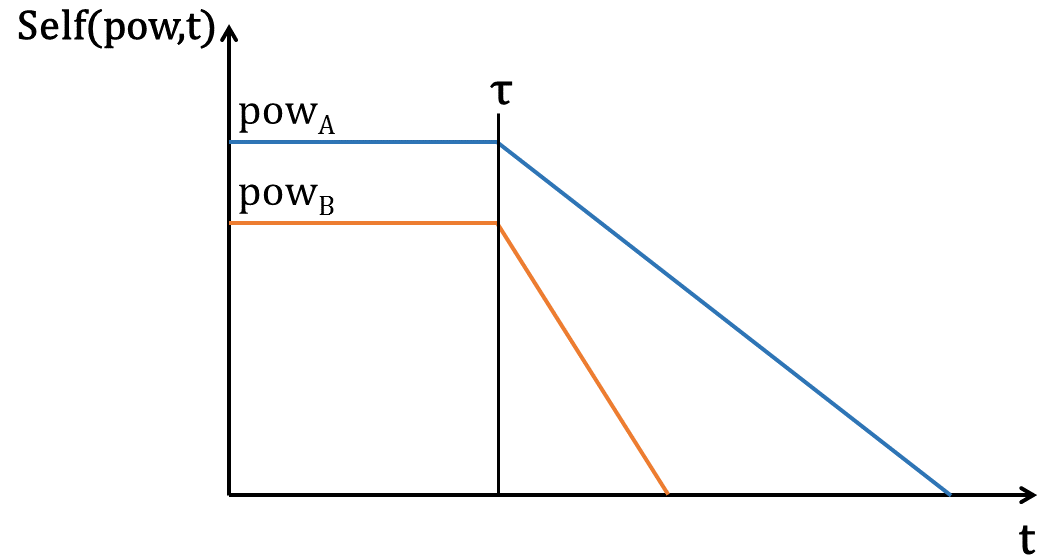
\includegraphics[width=2in]{Figures/sv3.png}
				\caption{\label{fig:conc}Courbe de concession reprenant le principe 1}
			\end{floatingfigure} 
			
	
	
	Concernant, les comportements de concession, nous avons élaboré une \emph {courbe de concession} illustrée sur la figure \ref{fig:conc}. 
	

	Soit $ self (dom, t) $ une fonction variant dans le temps, suivant la courbe de concession:
	\begin{equation}
	self(dom, t) = \left\{\begin{array}{ll}
	dom & \mathrm{if\ } (t \leq \tau)\\
	max(0, dom - (\frac{\delta}{dom} \cdot (t - \tau))) & \mathrm{otherwise}
	\end{array}\right.
	\end{equation}
	
	
	
	tel que :
	\begin{itemize}
		\item $t \geq 0$ est le nombre de propositions ouvertes ou rejetées ayant été exprimé durant la négociation.
		\item $\tau > 0$ le nombre minimal de propositions pour que les concessions commencent.
		\item  $\delta > 0$ un paramètre de calcul de la courbe de concession.
		
	\end{itemize}  
	
	La fonction $self(dom,t)$ représente le poids que l'agent attribut à sa satisfaction personnelle par rapport à la satisfaction de son partenaire de négociation. Plus la dominance de l'agent est élevée, plus son niveau d'exigence est important. Par ailleurs, la courbe de concession décroît plus rapidement pour des valeurs de dominance faibles.
	
	Ces comportements d'exigences et de concessions sont modélisés pour calculer l'acceptabilité d'une proposition 
	
	L'acceptabilité d'une valeur de critère $v \in C_i$ est défini comme une fonction booléenne:
	\begin{equation}
	\vspace{-.5em} 
	acc(dom,v, t) = sat_{self}(v, \prec_i) \geq  (\beta \cdot self(dom,t))
	\end{equation}
	
	\medskip
	où $\beta>0$ est un paramètre théorique qui définit le poids accordé au niveau d'exigence.
	
	cette fonction est généralisable aux options $o \in O$: $acc(dom,o, t) = sat_{self}(o, \prec) \geq  (\beta \cdot self(dom,t))$. Elle est utilisée afin de déterminer si une proposition est acceptable.
	
	
	
	
	\subsection {Prise en compte des préférences de soi Vs autrui}
	Selon notre second principe, les négociateurs dominants donnent plus de poids à leur propre satisfaction qu'a leur partenaires de négociation. 
	Pour implémenter ce principe dans le contexte de la négociation collaborative, nous calculons dans quelle mesure une proposition donnée est \emph{tolérable} pour la satisfiabilité de l'agent et de son partenaire.
	En effet, à chaque fois que l'agent énoncera une proposition, la valeur de cette dernière doit prendre en compte les préférences des deux interlocuteurs. 
	Donc, pour chaque critère $i\in\mathcal{C}$, considérons le sous ensemble $V_i\subseteq C_i$ de valeurs acceptables pour l'agent:

	\begin{equation}
	V_i(dom,t) = \{ v\in C_i : acc(dom,v,t) \}
	\end{equation}
	
	Cet ensemble correspond à toutes les propositions acceptables qu'un agent pourrait faire à un moment donné de la négociation.
	
	Nous calculons la tolérabilité d'une valeur donnée $ v \ dans V_i (dom, t) $ en équilibrant entre les préférences de l'agent et celles de son partenaire. Nous supposons que l'agent donne un poids à la satisfaction de son partenaire qui est complémentaire à son auto-satisfaction:
	
	\begin{equation}
	\begin{split}
	tol(v, t, \prec_i, A_i, U_i, dom) & = self(dom, t)  \cdot sat_{self}(v, \prec_i) \\
	& +  (1 - self(dom, t)) \cdot sat_{other}(v, A_i, U_i)
	\end{split} 
	\end{equation}
	

	Nous généralisons cette fonction à toute option $o=(v_1,\ldots,v_n) \in O$:
	
	\begin{equation}
	tol(o, t, \prec, A, U, dom) = \frac{ \sum_{i}^{n} tol(v_i, t, \prec_i, A_i, U_i, dom) } {n}
	\end{equation}
	
	\noindent
	Par conséquent, l'agent propose la valeur la plus \emph{tolérable} dans l'ensemble $V_i$:
	\begin{equation}
	propose(V_i, \prec_i,dom) =  \operatorname*{arg\,max}_{v \in V_i} ( tol(v))
	\end{equation}
	
	Par conséquent, plus l'agent est soumis, plus il va considérer les préférences de son interlocuteur.
	
	\subsubsection*{Résumé des paramètres computationnels}
	\begin{itemize}[noitemsep]
		
		\item $\pi \in $[0,1] : La frontière entre  les comportements soumis et dominants utilisé dans le choix d'un type d'acte de dialogue. (voir )
		\item $\tau > 0$ : le nombre minimal de propositions ouvertes ou rejetées avant le début de la concession.
		\item $\delta > 0$ : paramètre dans la pente de la courbe de concession.
		\item $\alpha> 0$: Le nombre maximums d'actes de dialogues informatifs consécutifs.
	\end{itemize}
	
	\subsection{Contrôle de la négociation}
	
	Le troisième principe stipule que les négociateurs dominants ont tendance à contrôler la négociation.
	Nous avons implémenté ce principe à travers un algorithme pour le choix de l'acte de dialogue à énoncer, comme présenté dans la table \ref{table:uttChoice}.
	
	Nous avons défini un seuil $\pi$  qui divise le spectre de dominance en deux, à savoir comportements dominant, où soumis.
	
	Prenant en compte trois paramètres; la valeur de dominance $dom$, l'acte de dialogue énoncé par le partenaire $u^{-1}$ et l'état courent de la négociation, l'agent sélectionne le premier acte dans la table \ref{table:uttChoice} dont la condition d'applicabilité est vérifiée.  
	
	
	Par exemple, un agent dominant mettra fin à la négociation dès que toutes les options restantes seront inacceptables (ligne 2). Un agent soumis rejettera et exprimera une \emph{State}, afin de justifier son refus et expliquer pourquoi la proposition n'est pas acceptable (ligne 14). S'il n'y a pas de proposition ouverte, l'agent avec un pouvoir faible demandera de nouvelles informations (ligne 18 -19).
	
	Dans notre modèle, un agent peut exprimer plusieurs actes de dialogues dans un même tour de parole. Ces cas sont représentés avec un signe $"+"$ dans la table \ref{table:uttChoice}.
	
	En fonction de la valeur de dominance, l'agent va adopter différentes stratégies dans la sélection de l'acte de dialogue à exprimer. En effet, dans les travaux en psychologie social, les négociateurs dominants se concentrent sur l'avancement de la tâche de négociation. Ceci ce traduit par le choix d'actes de négociations (ProposeValue /ProposeOption, RejectValue /RejectOption, AcceptValue/ AcceptOption) comme il est présenté dans les lignes (4 à 10).
	
	L'agent priorise les actes de négociations plutôt que les actes d'échanger d'informations sur les préférences. En effet, comme présenté à la ligne 3, après un nombre de tours $ \alpha $ consacrés au partage d'informations, l'agent fera plutôt des propositions que informer le partenaire de ses goûts. Un exemple est présenté dans le dialogue \ref{fig: ex-dialogue}.
	
	Au contraire, un négociateur soumis se concentrera sur la construction d'un modèle précis des préférences de son partenaire afin de prendre la décision la plus équitable. Il se concentrera plus sur \emph {actes d'échanges d'information} (StateValue ou AskValue / AskCriterion) comme le montre les lignes (18-20). De plus, les mouvements de négociation sont limités par des conditions qui garantissent que l'agent ait rassemblé suffisamment d'informations sur les préférences de son partenaire avant d'exprimer une proposition (ligne 16-17).
	
	\begin{table}[!t]
		
		\centering
		\begin{tabular}{|p{.5cm}|p{.9cm}|p{4cm}|p{7.5cm}|}
			\hline
			\parbox[t]{3mm}{\multirow{5}{*}{\rotatebox[origin=c]{90}{\centering \textbf{dom  $>\pi$}}}}&$N $de ligne& \textbf{Acte de dialogue} & \textbf{Condition} \\
			\cline{2-4}
			&1&NegotiationSuccess & $\exists o \in T\cup P$, $acc(dom,o,t)$ \\
			\cline{2-4}
			& 2& NegotiationFailure & $ \forall o \in \mathcal{O},  \neg acc(dom,o,t)$\\
			\cline{2-4}
			&3& StateValue(v) & $type(u^{-1}) = AskPreference \land n < \alpha$ \newline $n$ est le nombre d'actes informatifs successifs\\
			\cline{2-4}
			&4& AcceptValue(v)+ \newline ProposeValue(c) & $ \exists v \in P_i$ / $acc(dom,v,t) \land \exists i\in\mathcal{C}, acc(dom,c,t)$ \\
			\cline{2-4}
			&5& AcceptValue(v)+\newline ProposeOption(o) &  $ \exists v \in P_i$ / $ acc(dom,v,t) \land \exists o \in \mathcal{O}$/ $ v \in o \land acc(dom,o,t)$ \\
			\cline{2-4}
			&6& RejectValue(v)+\newline ProposeValue(c) & $ \exists v \in P_i$ / $ \neg acc(dom,v,t) \land \exists i\in\mathcal{C}, acc(dom,c,t)$ \\
			\cline{2-4}
			&7& RejectValue(v)+ \newline ProposeOption(o) &  $ \exists v \in P_i$ / $  \neg acc(dom,v,t) \land \exists o \in \mathcal{O}$/ $acc(dom,o,t)$ \\
			\cline{2-4}
			& 8&RejectOption($o_1$)+ ProposeOption($o_2$) & $ \exists o_1 \in P$ / $ \neg acc(dom,o_1,t) \land \exists o_2\in\mathcal{O}, acc(dom,o_2,t)$ \\
			\cline{2-4}
			&9& ProposeValue(v) & $\exists v \in C_i$ / $tol(v, t, \prec_i, A_i, U_i, dom)$\\
			\cline{2-4}
			&10& ProposeOption(o) & $\exists o \in \mathcal{O}$ / $tol(o, t, \prec_i, A_i, U_i, dom)$\\
			
			\hline
			
			\parbox[t]{2mm}{
				\multirow{5}{*}{\rotatebox[origin=c]{90}{ \textbf{dom  $ \leq \pi$}}}} & 11& Negotiation success &  $\exists o \in T$ \\
			\cline{2-4}
			&12& AcceptValue(v) & $\exists i\in\mathcal{C}, \exists v \in P_i, acc(dom, v, t)$ \\
			\cline{2-4}
			&13&AcceptOption(o) & $\exists o \in P, acc(dom, o, t)$ \\
			\cline{2-4}
			&14&RejectValue(v)+\newline StateValue(v) & $ t<\tau \land (\exists i\in\mathcal{C}, \exists v \in P_i, \neg acc(dom,v, t))$.\\
			\cline{2-4}
			&15&RejectOption(o)+ \newline StateValue(v) & $ t<\tau \land (\exists o \in P,  \neg acc(dom,o, t) \land \exists v \in o, \neg acc(dom,v, t))$.\\
			\cline{2-4}
			&16&ProposeValue(v) &  $\exists i\in\mathcal{C}, \exists v \in C_i, v \in A_i  \land acc(dom, v, t) $\\
			\cline{2-4} 
			&17&ProposeOption(o)  & $\forall i\in\mathcal{C},\exists v \in C_i, v \in T_i  \land v \in o$ \\
			\cline{2-4} 
			&18&AskValue(v) & $t > \tau \land \exists i\in\mathcal{C}, \exists c \in P_i, \neg acc(c, t)$ \\
			\cline{2-4} 	
			&19&AskCriterion(i) & $\exists i\in\mathcal{C}, A_i \cup U_i= \emptyset $\\
			\cline{2-4}	
			&20&StateValue(v) & $\exists i\in\mathcal{C}, C_i\cap S_i \neq \emptyset$	\\
			\cline{2-4}
			&21& ProposeValue(v) & $\exists v \in C_i$ / $tol(v, t, \prec_i, A_i, U_i, dom)$\\
			\cline{2-4}
			&22& ProposeOption(o) & $\exists o \in \mathcal{O}$ / $tol(o, t, \prec_i, A_i, U_i, dom)$\\
			
			\hline
		\end{tabular}
		
		\caption{Ordre de sélection d'actes de dialogues en fonction de la valeur de pouvoir}
		\label{table:uttChoice}
	\end{table}
	
			\colorbox{red}{AJOUTER UN DIALOGUE EXEMPLE AVEC LES VALEURS DE DOMINANCE}
	
	\section{Évaluation du modèle}
		
		Dans cette section, nous présentons une première évaluation de notre modèle de négociation collaborative. Cette dernière a pour objectif de valider l'implémentation de notre modèle de négociation collaborative et étudier la perception des comportements de dominance exprimés par l'agent au cours d'une négociation. 
		Pour ce faire, nous avons mené deux études, la première étude agent/agent où les participants avaient le rôle de juge externe pour évaluer le comportement des agents lors de leur négociation.
		La seconde étude visait à évaluer les comportements de l'agent au cours d'une interaction avec un utilisateur humain. Par conséquent, les participants ont négocié avec des agents pour ensuite évaluer leurs comportements. 
		
		\subsection{Hypothèses}
				
				Nous avons défini quatre hypothèses qui reflètent les différents comportements et stratégies affichés par les agents lors de la négociation. Dans ce qui suit, nous noterons l'agent qui exhibe des comportements dominants dans la relation interpersonnelle comme \emph{agent dominant}, et l'agent dans la position soumise comme \emph{l'agent soumis}.
				
				\begin{itemize}
					\item \textbf {H1:} L'agent dominant sera plus fortement perçu comme étant égocentrique que l'agent soumis.
					
					\item \textbf {H2:} L'agent dominant sera plus fortement perçu comme exigeant que l'agent soumis.
					
					\item \textbf {H3:} L'agent soumis sera perçu comme faisant des concessions plus importantes que l'agent dominant.
					
					\item \textbf {H4:} L'agent dominant sera plus fortement perçu comme prenant le contrôle de la négociation que l'agent soumis.
					
				\end{itemize}
				
		\subsection{Étude 1: Évaluation Agent/Agent}
				L'objectif de cette étude est d'analyser la perception des différents comportements de dominance qui peuvent apparaître au cours d'une négociation. En effet, chaque comportement implémenté est lié à un principe et donc indépendant des autres principe. Nous visons donc à étudier si les différents comportements de l'agent durant la négociation vont être correctement associé à des comportements de dominance. Pour ce faire, nous avons généré des dialogues entre deux agents doté de notre modèle de négociation. 
			
			\subsubsection{Implémentation des agents négociateurs}
				Nous avons implémenté deux agents qui devaient simuler une relation interpersonnelle de dominance. Pour ce faire, un agent a été initialisé pour produire des comportements dominants et l'autre agent produisait des comportements complémentaire de soumission. 
				
				
				Nous avons manipulé des paramètres de simulations afin d'initialiser les comportements des deux agents.
				
				Premièrement, nous avons fixé les paramètres computationnels de nos fonctions de décisions: $\tau=2$, $\pi=0.5$, $\alpha=2$, $\beta=1$ et $\delta=0.1$. 
				Deuxièmement, nous avons choisi les valeurs de dominance $dom$ de chaque agent afin de le positionner dans le spectre de dominance. 
				Ensuite, nous avons défini les préférences de chaque agent. En effet, les préférences ont un impact direct sur le processus de décision, il fallait donc générer des préférences différentes qui vont stimuler le processus de décision. Pour cela, nous avons utilisé la mesure de distance \emph{Kendall tau} \cite{bra2013Kendall} qui permet de calculer la distance entre deux ensembles de préférences d'ordre partiel. 
				Nous présentons dans ce qui suit la définition de la distance de Kendall. 
				
				\vspace{1 em}
				\textbf{Définition. }
%				\vspace{0.75 em}
				La distance de Kendall considère les distances entre deux ordres partiels en fonction de leurs ensembles d'extensions totales.
				
				Pour chaque ensemble partiel, l'algorithme génère des extensions de cet ensemble jusqu'à arriver à un des ordre total. Pour un ensemble $\sigma$, nous notons l'ensemble des extensions possibles de ce modèle $ext(\sigma)$.
				
				La distance entre deux modèle partiels  $\sigma$ et $\mu$ est donc calculé comme suit: 

				
				\begin{equation*}
					K_H(\sigma,\mu) = max \left \{ \max\limits_{\alpha \in ext(\sigma)} \min\limits_{\beta \in ext(\mu)} K(\alpha , \beta), \max\limits_{\beta \in ext(\mu)} \min\limits_{\alpha \in ext(\sigma)} K(\beta, \alpha)  \right \}
				\end{equation*}
				
				tel que $K(\alpha , \beta)$ est la distance entre les deux ensembles d'ordre totaux $\alpha$ et $\beta$ qui compte le nombre les désaccords ou des inversions de paires de préférences entre les deux ensembles. 
				 
				
				Enfin, nous avons défini le sujet de négociation. Nous avons opté pour un sujet social qui n'exige pas de compétence techniques. Les négociateurs avait pour but de négocier afin de choisir un restaurant. Nous avons pris en compte quatre critères pour le choix d'un restaurant. 	Les critères sélectionnés sont \ {\textit {cuisine, prix, ambiance, emplacement} \}. Chaque critère a été défini avec un domaine de valeurs, et un total de 420 restaurants a été généré à partir des valeurs de chaque critère.
				
				
				Au final, nous avons obtenu quatre conditions expérimentales résumées dans la table \ref{table:conditions}. Nous avons généré un dialogue par condition (pour un total de 4 dialogues). Les dialogues générés sont disponibles en Appendixe ...
				
				\begin{table}[b]
					\centering
					\begin{tabular}{ |l|c|c|l| }
						\hline
						\textbf{Préférences}& \textbf{A} & \textbf{B} & \textbf{Label} \\ 
						\hline
						\newline\multirow{3}{*} {Préférences distantes (Kendall's tau = $0.96$)} & 0.9 & 0.4 & Dialogue 1 \\ \cline{2-4}
						
						\newline  & 0.7 & 0.4 & Dialogue 2\\ \cline{2-4}
						
						\newline   &0.7 & 0.2 & Dialogue 3\\ 
						\hline
						\newline Préférences similaire (Kendall's tau = $0.46$) & 0.7 & 0.4 & Dialogue 4\\
						\hline
					\end{tabular}
					\caption{Conditions expérimentales pour la génération des dialogues.} 
					\label{table:conditions}
				\end{table}
		
			\subsubsection{Procédure}
					We conducted a between-subject study using the online crowdsoursing website \emph{CrowdFlower}\footnote{https://www.crowdflower.com/}. 
					Each participant was shown only one dialogue. Speaker A and B were described as two friends trying to negotiate a restaurant to have dinner. %We wanted to avoid skewing the participant's perception by the fact that negotiators are artificial agents. 
					Participants were asked to read the assigned dialogue and answer a questionnaire. 
					
					We defined two questions for each hypothesis. Two test questions were included to check the	sanity of the answers. We eliminated participants providing wrong answers to those questions. Each one of these questions was to be answered on a 5 points Likert scale ranging from ``I totally disagree" to ``I totally agree".
			
			\subsubsection{Résultats}
			
			\subsubsection{Discussion}	
				